\documentclass[]{report}
\usepackage{lmodern}
\usepackage{amssymb,amsmath}
\usepackage{ifxetex,ifluatex}
\usepackage{fixltx2e} % provides \textsubscript
\ifnum 0\ifxetex 1\fi\ifluatex 1\fi=0 % if pdftex
  \usepackage[T1]{fontenc}
  \usepackage[utf8]{inputenc}
\else % if luatex or xelatex
  \ifxetex
    \usepackage{mathspec}
  \else
    \usepackage{fontspec}
  \fi
  \defaultfontfeatures{Ligatures=TeX,Scale=MatchLowercase}
\fi
% use upquote if available, for straight quotes in verbatim environments
\IfFileExists{upquote.sty}{\usepackage{upquote}}{}
% use microtype if available
\IfFileExists{microtype.sty}{%
\usepackage{microtype}
\UseMicrotypeSet[protrusion]{basicmath} % disable protrusion for tt fonts
}{}
\usepackage[left=3cm,right=3cm,top=2cm,bottom=2cm]{geometry}
\usepackage{hyperref}
\hypersetup{unicode=true,
            pdfauthor={Samuel Lippl},
            pdfborder={0 0 0},
            breaklinks=true}
\urlstyle{same}  % don't use monospace font for urls
\usepackage{natbib}
\bibliographystyle{apalike}
\usepackage{longtable,booktabs}
\usepackage{graphicx,grffile}
\makeatletter
\def\maxwidth{\ifdim\Gin@nat@width>\linewidth\linewidth\else\Gin@nat@width\fi}
\def\maxheight{\ifdim\Gin@nat@height>\textheight\textheight\else\Gin@nat@height\fi}
\makeatother
% Scale images if necessary, so that they will not overflow the page
% margins by default, and it is still possible to overwrite the defaults
% using explicit options in \includegraphics[width, height, ...]{}
\setkeys{Gin}{width=\maxwidth,height=\maxheight,keepaspectratio}
\IfFileExists{parskip.sty}{%
\usepackage{parskip}
}{% else
\setlength{\parindent}{0pt}
\setlength{\parskip}{6pt plus 2pt minus 1pt}
}
\setlength{\emergencystretch}{3em}  % prevent overfull lines
\providecommand{\tightlist}{%
  \setlength{\itemsep}{0pt}\setlength{\parskip}{0pt}}
\setcounter{secnumdepth}{5}

%%% Use protect on footnotes to avoid problems with footnotes in titles
\let\rmarkdownfootnote\footnote%
\def\footnote{\protect\rmarkdownfootnote}

%%% Change title format to be more compact
\usepackage{titling}

% Create subtitle command for use in maketitle
\providecommand{\subtitle}[1]{
  \posttitle{
    \begin{center}\large#1\end{center}
    }
}

\setlength{\droptitle}{-2em}

  \title{}
    \pretitle{\vspace{\droptitle}}
  \posttitle{}
    \author{Samuel Lippl}
    \preauthor{\centering\large\emph}
  \postauthor{\par}
      \predate{\centering\large\emph}
  \postdate{\par}
    \date{2019-08-14}

\usepackage{booktabs, titlesec, blindtext}
\usepackage[svgnames]{xcolor}
\hypersetup{
    bookmarksnumbered=true,
    bookmarksopen=false,
    bookmarksopenlevel=1,
    colorlinks=false,
    linkcolor=blue,
    urlcolor=DarkBlue,
    citecolor=blue
}
\definecolor{chgray}{gray}{0.5}
\newcommand{\hsp}{\hspace{20pt}}
\titleformat{\chapter}[hang]{\Huge\bfseries}{\thechapter\hsp\textcolor{chgray}{|}\hsp}{0pt}{\Huge\bfseries}
\normalfont
\usepackage{setspace}
\usepackage{subfig}

\usepackage{amsthm}
\newtheorem{theorem}{Theorem}[chapter]
\newtheorem{lemma}{Lemma}[chapter]
\theoremstyle{definition}
\newtheorem{definition}{Definition}[chapter]
\newtheorem{corollary}{Corollary}[chapter]
\newtheorem{proposition}{Proposition}[chapter]
\theoremstyle{definition}
\newtheorem{example}{Example}[chapter]
\theoremstyle{definition}
\newtheorem{exercise}{Exercise}[chapter]
\theoremstyle{remark}
\newtheorem*{remark}{Remark}
\newtheorem*{solution}{Solution}
\begin{document}

\begin{titlepage}

% Titlepage inspired by: https://www.overleaf.com/15991102jmmvbxxtbhfk#/61015645/

\newcommand{\HRule}{\rule{\linewidth}{0.5mm}} % Defines a new command for the horizontal lines, change thickness here

\center % Center everything on the page

%----------------------------------------------------------------------------------------
%	TITLE SECTION
%----------------------------------------------------------------------------------------

\HRule \\[0.4cm]
{ \huge \bfseries Creating Novel Sensorimotor Responses in Auditory Cortex}\\[0.4cm] % Title of your document
\HRule \\[1.5cm]


%----------------------------------------------------------------------------------------
%	HEADING SECTIONS
%----------------------------------------------------------------------------------------

\textsc{\LARGE University of Oxford}\\[0.5cm] % Name of your university/college
\textsc{\Large Department of Physiology, Anatomy, and Genetics}\\[1.5cm]


\textsc{\Large MSc Neuroscience}\\[0.5cm] % Major heading such as course name
\textsc{\large Trinity Term 2019\\Dissertation 2}\\[0.5cm] % Minor heading such as course title

%----------------------------------------------------------------------------------------
%	LOGO SECTION
%----------------------------------------------------------------------------------------

\vfill


\includegraphics[height=0.2\textheight]{figs/ox_sigil.eps}\\[1cm] % Include a department/university logo - this will require the graphicx package



%----------------------------------------------------------------------------------------
%	DATE SECTION
%----------------------------------------------------------------------------------------

\vfill

%----------------------------------------------------------------------------------------
%	AUTHOR SECTION
%----------------------------------------------------------------------------------------

\begin{Large}
\textsc{Candidate Number}\\1030208\\[1cm]
\textsc{Word Count}\\8123\\[1cm]
\textsc{Supervisors}\\
\begin{tabular}{cc}
Samuel Picard&
Yves Weissenberger\\
Andrew King&
Johannes Dahmen
\end{tabular}
\end{Large}

\vfill

\end{titlepage}

\pagenumbering{roman}
\setcounter{page}{2}

\doublespacing
\begin{abstract}

Relating motor output to its sensory consequences is critical to navigating complex environments. In order to investigate the emergence of artificial sensorimotor contingencies, we trained mice on a novel sensorimotor task that required them to navigate through a virtual tonespace while recording from large numbers of neurons in auditory cortex using 2-photon imaging. Five out of nine mice learned the sensorimotor contingency and in an example session of one of those mice, a small proportion of neurons was sensitive to violations of the contingency. The task and its variations connect a simple behavioural paradigm in head fixed mice to some of the most debated computational theories of learning, producing neural and behavioural data that can be used to test their predictions. 


\end{abstract}

\tableofcontents

\hypertarget{intro}{%
\chapter{Introduction}\label{intro}}

\pagenumbering{arabic}
\setcounter{page}{1}

Relating motor output to its sensory consequences is critical to simple
movements and more complex behaviour. In the case of innate sensorimotor
contingencies, the brain is thought to make use of corollary discharges,
which cancel out the sensory consequence of a motor action by
subtracting its predicted effect from the sensory input and play an
important role even in simple circuits \citep{poulet2003cricket}.
Whether they are mediated by elementary computations or require more
finely tuned control, these corollary discharges demonstrate the
existence and usefulness of a generative model of sensorimotor
contingencies \citep{miall1996forward}. These innate contingencies are
also represented in sensory areas of the cortex where neurons signal the
mismatch between visual input and predicted visual flow
\citep{keller2012sensorimotor, leinweber2017sensorimotor}, and between
vocalizations and auditory feedback \citep{eliades2018auditory}.

While the representation of innate sensorimotor contingencies is
important for everyday behaviour, it is equally important to be able to
recognize novel contingencies in dynamically changing environments.
Humans and animals are adept at extracting statistical information from
volatile environments \citep{behrens2007information}. This is mediated,
in part, by sensory areas of the cortex, which are thought to construct
a model of their environment \citep{berkes2011spontaneous}. In
particular, some neurons respond more strongly to unexpected stimuli.
For example, neurons in auditory cortex encode oddballs, tones that are
unlikely according to the recent history of stimulus presentation
\citep{gill2008surprise, rubin2016representation}. This model guides how
multisensory as well as sensorimotor information is integrated
\citep{gallistel2001rat, ernst2002humans, kording2004force, kording2004bayesian}.

In contrast to statistical patterns in the environment, artificial
sensorimotor contingencies take the observer into account as a causal
actor. Such contingencies are abundant in our daily lives, in particular
in light of technological advancement, but it is advantageous for many
animals to learn such novel rules, as well. Relatively little research
has been carried out on this. However, \citet{aronov2017grid} found that
training rats to manipulate the frequency of a presented sound by
pressing a lever resulted in the induced virtual tonespace being
represented in a grid cell-like fashion in the hippocampal-entorhinal
circuit. Furthermore, it has been shown that neurons in auditory cortex
suppress artificial sensory consequences of movement when mice are
passively presented with such a contingency
\citep{schneider2018cortical}.

In order to investigate the emergence of novel, behaviourally relevant
sensorimotor contingencies, we trained mice to manipulate stimulus
frequency by their licking behaviour while recording from large numbers
of neurons in auditory cortex using 2-photon imaging. Mice were
presented with tones at a regular interval and position in front of two
spouts. Licking one of them led to a decrease in frequency of the
presented tones, licking the other one led to an increase in frequency.
In accordance with this contingency, the mice had to navigate to a
rewarded frequency region in order to receive a drop of water. In this
dissertation, I am going to investigate whether the mice were able to
learn this task and what effect the presented contingency had on the
activity of neurons in auditory cortex.

\hypertarget{methods}{%
\chapter{Methods}\label{methods}}

\hypertarget{animals}{%
\section{Animals}\label{animals}}

\hypertarget{strain}{%
\subsection{Strain}\label{strain}}

All experiments were approved by the local ethical review committee at
the University of Oxford and licensed by the UK home office. Eleven mice
(three male (M01-03) and eight female (M04-11)) were used for the
behavioural experiments. They came from a line obtained by crossing the
floxed-Ai95 (RCL-GCaMP6f)-D line (Jackson Laboratories; stock number
024105) with the CaMKIIalpha-Cre T29-1 line (Jackson Laboratories; stock
number: 005359). As a result, the mice expressed the fluorescent calcium
indicator GCaMP6f \citep{chen2013gcamp} in cortical excitatory neurons.

\hypertarget{surgeries}{%
\subsection{Surgeries}\label{surgeries}}

At five to ten weeks of age, each animal was implanted with a metal head
post and a cranial glass window over right auditory cortex, using
surgical procedures described previously \citep{weissenberger2019licks}.
Briefly, after inducing general anaesthesia through the inhalation of
isoflurane, the animal was placed in a stereotactic frame (Model 900LS,
David Kopf Instruments). Body temperature and anaesthetic depth were
monitored and kept constant throughout the surgery. The eyes were
lubricated with eye ointment. Under aseptic conditions, the hair over
the skull was removed. Following an incision into the scalp and the
removal of the surrounding tissue, a 4mm circular craniotomy was drilled
over right auditory cortex and a custom-made cylindrical window was
placed onto the brain and glued to the surrounding skull.
Post-operatively, the animals were given analgesia, kept warm, and
monitored for at least 48 hours. All mice were allowed to recover for at
least one week after surgery.

\hypertarget{preparations-for-behavioural-training}{%
\subsection{Preparations for behavioural
training}\label{preparations-for-behavioural-training}}

After recovery, the mice were restricted to 1 ml of water per day in
preparation of the behavioural training. Throughout the water
restriction, the animal's weights were measured relative to their
initial weight on a daily basis. Weight loss was kept constant around
85\% and not allowed to fall under 80\%. Behavioural training began
after the weight had stabilized.

\hypertarget{materials}{%
\section{Materials}\label{materials}}

\hypertarget{behavioural-setup}{%
\subsection{Behavioural setup}\label{behavioural-setup}}

Mice M01-M07 were pre-trained in behavioural boxes before being imaged
under the microscope, whereas mice M08-M11 were trained under the
microscope setup from the beginning. For these purposes, several
two-spout lick detection circuits were built following the diagram by
\citet{slotnick2009lick}. The mice were positioned in a conductive tube
that was connected to this circuit. When they licked the spouts, which
were also connected, they closed this circuit, which was registered.

In the behavioural boxes, the task was controlled using a custom-written
program in Python 2 \citep{python} using the packages `numpy'
\citep{oliphant2006numpy, vanderwalt2011numpy}, `random', `time',
`multiprocessing', `RPi.GPIO', `csv', `requests', `pygame', and `sys'.
This program was executed on a Raspberry Pi 2 that was connected to the
lick detection circuits and a solenoid responsible for delivering
rewards in the form of 0.005ml drops of water.

In the microscope setup, the task was controlled using a custom-written
program in Matlab 2017b (© Mathworks), which was connected to the task
setup by a 10 MHz data acquisition board (National Instruments). This
allowed for synchronization of the behavioural data with the microscope
frame clock. Sound presentation was mediated using Psychtoolbox V3
\citep{brainard1997psychtoolbox, pelli1997psychtoolbox, kleiner2007psychtoolbox}.
The levels of the presented sound were calibrated with a free-field
high-frequency microphone (GRAS), and the latency of the sound
presentation was determined and corrected for in the analysis.

Each animal performed the behavioural task once a day using between one
and six blocks of training. Overall, this yielded 97 blocks of
behavioural data from the box setup and 618 blocks of behavioural data
from the microscope setup. Of these 618 blocks, imaging data was
acquired on 233 blocks.

\hypertarget{two-photon-imaging-setup}{%
\subsection{Two-photon imaging setup}\label{two-photon-imaging-setup}}

Calcium imaging of auditory cortex was performed as described in
\citet{weissenberger2019licks}, using a rotating two-photon
laser-scanning microscope (Bergamo II, Thorlabs) with a 20x/1.00
immersion objective (Olympus). Excitation light (940 nm) was emitted
from a femtosecond laser (Chameleon Discovery, Coherent) at 1250 mW,
attenuated with a neutral density filter wheel (Thorlabs), and
amplitude-modulated with a Pockels cell (302RM, Conoptics). This beam
was then optically expanded and guided through a periscope into the
scanhead where it was scanned onto the brain with an 8kHz resonant
scanner and a galvanometric scan mirror, enabling the acquisition of
512x512 pixel frames at rates of 29.7 Hz. The microscope was controlled
using ScanImage 2017 (Vidrio Technologies).

\hypertarget{widefield-imaging-setup}{%
\subsection{Widefield imaging setup}\label{widefield-imaging-setup}}

Widefield calcium imaging allowed for the identification of putative
functional areas of auditory cortex. Before starting behavioural
training, animals were head-fixed and passively exposed to a repeating
sequence of eight different sinusoidally amplitude modulated (SAM) tones
(4, 5, 25 \& 32 kHz; 55 \& 65 dB SPL; 500 ms duration; 10 Hz modulation
frequency; 100\% modulation depth; 15 repeats) . Images were acquired at
10 Hz through a TL2x-SAP objective (Thorlabs) and a 340M-GE camera
(Thorlabs) using a blue LED for widefield excitation. Evoked responses
to SAM tones were averaged (1-10 frames post-onset) and baseline
corrected (1-6 frames pre-onset), and resulting response amplitude maps
were plotted for each frequency-level combination. Based on the quality
of the response maps, one pair of average low- and high-frequency
SAM-responses was chosen for computing the widefield map. Two-photon
images were registered to the widefield map by visually aligning the
blood vessel pattern to the mean widefield image.

\hypertarget{imaging-procedures}{%
\subsection{Imaging procedures}\label{imaging-procedures}}

To record from neurons in the auditory cortex, the animals were head
fixed in an optically and acoustically isolated imaging booth. During
the subsequent imaging preparations, they performed the behavioural
task. As a reference position, the microscope was positioned at the
surface of the brain and the center of the widefield image. This allowed
us to move the microscope to the functional areas of auditory cortex
that had been identified using widefield calcium imaging and to find the
same areas again across different days. Imaging was performed at planes
of 170-250 µm below the surface, corresponding to cortical layers 2/3.

Subsequently, suitable areas for imaging were identified using the
functional areas identified by the widefield image, the visibility of
the neurons in these areas, and the robustness of their auditory
responses. Several areas were recorded on different days to sample from
different areas within auditory cortex. After selecting three to four
locations in such a manner, these areas were repeatedly imaged
throughout the remaining days as long as visibility allowed it. The same
imaging location was determined using the reference frame and the brain
surface, as well as a mean image of the recorded area to align the
microscope between several days.

Imaging blocks of 10 minutes were acquired consecutively as long as the
animal behaved sensibly, but never for longer than an hour. In this
manner, imaging data were collected for 233 blocks, in total.

\hypertarget{behavioural-paradigm}{%
\section{Behavioural paradigm}\label{behavioural-paradigm}}

\hypertarget{sensorimotor-task}{%
\subsection{Sensorimotor task}\label{sensorimotor-task}}

The mice were head fixed in front of two spouts that were positioned
either side of their snout. Sometimes the spouts were shifted to one
side to counteract a bias into one direction. The mice were presented
every 500 ms with pure tones that were 200 ms long and between 60 and 65
dB. These tones were centered around 11.3kHz and arranged in six steps
per octave. When they were presented with stimuli spanning one octave,
these were logarithmically arranged in the space between 8 and 16 kHz. A
three octaves space spanned the range from 4 to 32 kHz. By licking the
two spouts in front of them, the mice manipulated the frequency that was
presented next. For this purpose, the counts nr and nl of right and left
licks respectively were determined in either a window of 700 to 200ms or
a window of 600 to 100ms before the next stimulus presentation. The
current stimulus frequency was subsequently shifted by steps that were
determined by rounding the formula

\[2\left(\log(n_r+1)-\log(n_l+1)\right)\]

to the nearest whole number. These shifts were bounded by the number of
octaves in a given trial. Mice were presented either with an
RL-contingency such that right licks led to a decreasing stimulus
frequency and left licks led to an increasing frequency, or an
LR-contingency, in which left and right licks led to decreasing and
increasing frequencies, respectively.

When the tone frequency was at most one step away from the middle
frequency (i. e. between 10 and 12kHz), mice were presented with a small
drop of water (0.005ml) in the spout they had last licked. In order to
reach this rewarded region, the stimuli outside of this rewarded region
therefore implied the strategy that needed to be employed in order to
reach the rewarded region. In the RL-contingency (resp. LR-contingency),
frequencies above (resp. below) the rewarded region implied a
`Rightwards!' strategy, where the animal needed to lick right, and
frequencies below (resp. above) the rewarded region implied a
`Leftwards!' strategy, where the animal need to lick the left spout (see
figure \ref{fig:a-example-py} for an example of an RL-contingency).

Recorded licks and rewards as well as presented sounds were registered
in a text file for offline analysis.

\hypertarget{violations-of-the-contingency}{%
\subsection{Violations of the
Contingency}\label{violations-of-the-contingency}}

For the purpose of understanding whether the mice had learned the
sensorimotor contingency, and whether auditory cortex represented this
contingency, targeted violations of the contingency were introduced to
decouple sensorimotor dynamics from its confounding factors. When the
lick rate was non-zero, random jumps in tone frequency were occasionally
being presented, violating the sensorimotor contingency.

Larger jumps led to perturbations in strategy. Without such
perturbations, a sound-driven policy would lead to a motor pattern of
alternating left and right lick bouts. Such a policy would be
indistinguishable from a policy based on a regular motor pattern
switching between left and right lick bouts. After a strategy
perturbation, an animal implementing a motor-driven policy should employ
the same lick pattern as if the perturbation had not occurred, whereas
an animal implementing a sound-driven policy should adapt its behaviour
accordingly. By comparing the licking behaviour after such an event with
the regular licking behaviour, a sound-driven policy could therefore be
distinguished from a motor-driven policy. For this purpose, jumps were
generate from a uniform distribution including all possible changes.

These large jumps were apparent as sensory oddballs. In the case of
smaller jumps, the tones could be matched with tones following the
regular contingency for their frequency and sound history (going back
one stimulus). If the recorded neurons reacted differently to those
tones violating the sensorimotor contingency, this would therefore
indicate that these neurons represented the sensorimotor contingency.
For this purpose, jumps were randomly generated from the prior
distribution of stimulus changes.

\hypertarget{sound-level-modulations}{%
\subsection{Sound level modulations}\label{sound-level-modulations}}

Cortex has been demonstrated in multiple areas to integrate multimodal
information according to their respective precision
\citep{kording2004bayesian}. In order to probe the integration of
sensory and motor evidence sound levels were decreased by 20 dB in some
sessions to manipulate their precision. In these sessions, every
stimulus had an equal probability of being represented at a sound level
of 40-45 dB or 60-65 dB.

\hypertarget{training-methods}{%
\subsection{Training Methods}\label{training-methods}}

In the beginning, the mice were rewarded for licking the spouts to guide
their behaviour into the correct direction. Subsequently, they were
presented with a simple version of the behavioural paradigm, where the
sounds were presented within one octave and without perturbations. As
the animals' behaviour stabilized this window was extended to two and
finally three octaves and strategy perturbations were introduced. To
guide their behaviour in the initial stages, rewards were presented
outside of the rewarded frequencies if either of the following
conditions was satisfied: 1) the animal licked after having not licked
for two minutes; 2) the animal licked in the direction that moved it
closer to the rewarded frequency region after having not received a
reward for ninety seconds. These rewards were omitted from the analysis.

\hypertarget{imaging-procedures-1}{%
\subsection{Imaging procedures}\label{imaging-procedures-1}}

To record from neurons in the auditory cortex, the animals were head
fixed in an optically and acoustically isolated imaging booth. During
the subsequent imaging preparations, they performed the behavioural
task. As a reference position, the microscope was positioned at the
surface of the brain and the center of the widefield image. This allowed
us to move the microscope to the functional areas of auditory cortex
that had been identified using widefield calcium imaging and to find the
same areas again across different days. Imaging was performed at planes
of 170-250 µm below the surface, corresponding to cortical layers 2/3.

Subsequently, suitable areas for imaging were identified using the
functional areas identified by the widefield image, the visibility of
the neurons in these areas, and the robustness of their auditory
responses. Several areas were recorded on different days to sample from
different areas within auditory cortex. After selecting three to four
locations in such a manner, these areas were repeatedly imaged
throughout the remaining days as long as visibility allowed it. The same
imaging location was determined using the reference frame and the brain
surface, as well as a mean image of the recorded area to align the
microscope between several days.

Imaging blocks of 10 minutes were acquired consecutively as long as the
animal behaved sensibly, but never for longer than an hour. In this
manner, imaging data were collected for 233 blocks, in total.

\hypertarget{reproducibility}{%
\section{Reproducibility}\label{reproducibility}}

The collected behavioural and neural data is available in the Python
package `toneworld', which was created for the purpose of this
dissertation and also contains the behavioural and neural analysis
pipeline. A small showcase of its functionality can be found in the
appendix. The package relied on the packages `copy', `numpy', `pandas'
\citep{pandas}, `setuptools', `tqdm', `math', `scipy' \citep{scipy},
`bootstrapped', and `plotnine'. Parts of the analysis specific to this
dissertation were conducted in R \citep{R-base} using the packages
`broom' \citep{R-broom}, `dplyr' \citep{R-dplyr}, `feather'
\citep{R-feather}, `ggplot2' \citep{R-ggplot2}, `grid', `lubridate'
\citep{R-lubridate}, `magrittr' \citep{R-magrittr}, `muStat'
\citep{R-muStat}, `png' \citep{R-png}, `reticulate'
\citep{R-reticulate}, `stringr' \citep{R-stringr}, and `tidyr'
\citep{R-tidyr}. The dissertation itself was written in R using
`bookdown' \citep{R-bookdown}, `knitr' \citep{R-knitr}, and `rmarkdown'
\citep{R-rmarkdown}. The package and the code necessary to reproduce the
dissertation is available upon request.

\hypertarget{behavioural-analysis}{%
\section{Behavioural analysis}\label{behavioural-analysis}}

In order to analyze the mice's behaviour, the lickrates before and after
certain sound events were determined. For this purpose, only changing
sounds were included to omit behaviorally inactive phases. When a sound
changed from a frequency region that suggested one particular strategy
to a region that suggested another strategy, this warranted a change in
licking behaviour according to a sound-driven policy. Using bins of 250
ms, the average lickrates in a five second window before and after such
a strategy event were therefore assessed.

Subsequently, the effect of strategy perturbations was analysed by
comparing violations of the paradigm that led to perturbations to those
that did not. Mann-Whitney U tests \citep{hodges1956nonparametric} were
used to assess the nully hypothesis that the lick rate either did not
change or changed into the wrong direction.

This analysis was summed up by determining the change in lickrate
difference induced by the sound events. For this purpose, the difference
between the right and left lick rate in the second before and after
stimulus onset was determined. The lickrate difference before stimulus
onset was then subtracted from the lick rate difference after onset. A
positive (resp. negative) change in lick rate difference thus implied
that the corresponding sound event led to a higher proportion of right
(resp. left) licks.

The Prentice-Wittkowski test
\citep{prentice1979test, wittkowski2007test} is a generalization of the
Wilcoxon rank-sum test that allows for between-group comparisons within
blocks of unequal length. This test was used to assess the null
hypothesis that in a random stimulus event, the change in lickrate
difference was not positive where it should be positive and not negative
where it should be negative. Events were blocked according to the day,
and the previous strategy. The p-value was then determined for each
mouse individually.

The course of behavioural learning in mouse M10 was first assessed by
comparing the reactions to strategy perturbations on days one to seven
to the reactions on days fourteen to twenty using the framework
involving the Mann-Whitney U test and the Prentice-Wittkowski test
described above.

Behavioural analysis was restricted to the sessions under the imaging
setup. Due to a damaged headbar, mouse M05 could not continue its
behavioural training in this environment. Behavioural data of mouse M02
suggested that the data collection had been corrupted. Both animals were
therefore excluded from analysis. Including the corrupted data from M02
did not change the results of the Prentice-Wittkowski test across all
animals.

\hypertarget{neural-analysis}{%
\section{Neural Analysis}\label{neural-analysis}}

The Suite2p package \citep{pachitariu2017suite2p} was used to preprocess
the neural data, extract fluorescence traces and infer spike rates.
Preprocessing involved registration of the image frames to a 100-frame
mean image using efficient subpixel registration methods
\citep{guizar2008subpixel}, SVD decomposition and region of interest
(ROI) detection. A classifier was used to select neurons from the
candidate ROIs. The default classifier for this purpose was fine tuned
by manual assessment for the first few sessions, considerably improving
its performance. Finally, the spike-rates of these neurons were
determined using the OASIS algorithm implemented in suite2p. This
included classifying which of these regions of interest corresponded to
actual neurons. The classifier for this purpose was fine tuned by manual
assessment for the first few sessions and improved its performance based
on these data. Finally, the spike-rates of these neurons were determined
using the deconvolution algorithm included in `suite2p'.

The auditory response of these neurons was determined by determining
their spike-rate for the different tone frequencies in the 300 ms after
stimulus onset. Since the stimulus lasted for 200 ms, this spike-rate
included both onset and offset responses. Due to sensory adaptation,
neurons generally react more strongly to changing stimuli
\citep{westerman1984rapid}. For this reason, only changing tones were
included in this analysis. Using a Kruskal-Wallis-test, a nonparametric
analysis of variance \citep{kruskal1952}, neurons were identified whose
responses significantly differed across the presented frequencies
(\(p<0.0001\)). Only these neurons were included in the subsequent
analysis. The best frequency was determined as the frequency that, on
average, elicited the highest spike-rate.

As a next step, a Prentice-Wittkowski test was used to determine whether
compared to regular sounds, the neural response significantly differed
for events that violated the sensorimotor contingency, but were matched
in the manner described above. This was first assessed on a population
response, resulting in a single p-value. As a next step, this test was
applied to every single neuron, resulting in a distribution of p-values.
By shuffling the perturbations across events, the distribution of these
p-values was determined under the null hypothesis that pure sensorimotor
perturbations did not elicit different spike-rates in any neuron and
compared to the true distribution of p-values.

\hypertarget{results}{%
\chapter{Results}\label{results}}

\hypertarget{acquisition}{%
\section{Acquisition}\label{acquisition}}

This section discusses the behavioural evidence that the mice have
learned the sensorimotor contingency. For the purpose of this analysis,
this is assumed to be the case if the mice adapt their behaviour in a
sensible and sound-driven manner, i. e. animals should lick in a manner
that would bring the presented stimulus closer to the rewarded region.
In particular, it is not sufficient if their behaviour can be explained
by a behavioural policy that is based on a regular motor pattern that is
independent of the sounds. It is possible to distinguish a sound-driven
policy from such a motor-driven policy using the two groups of stimuli
presented below. Based on these groups and focussing on mouse M10, the
subsequent sections will discuss the acquisition of the contingency in
all animals and the course of learning in M10 alone.

\hypertarget{distinguishing-a-sound-driven-policy-from-a-motor-driven-policy}{%
\subsection{Distinguishing a sound-driven policy from a motor-driven
policy}\label{distinguishing-a-sound-driven-policy-from-a-motor-driven-policy}}

The following paragraphs are going to explain how targeted variations of
the task paradigm can distinguish a sound-driven policy from a policy
based on learned motor patterns.

At any given time, the spout the animal should lick is determined by the
sounds the animal is hearing. In the excerpt shown in figure
\ref{fig:a-example-py}, initially the sounds are above the rewarded
region, therefore the animal must lick right in order to reach the
rewarded region. (Henceforth, such stimuli are called `Rightwards!'
sounds.) As the animal employs the correct strategy and licks right, it
reaches the rewarded region and is thus presented with a drop of water.
As it keeps licking the right spout, the correct strategy changes to
`Leftwards!'. The mouse switches its lick pattern and is therefore
rewarded. Subsequently, the stimulus again changes to a `Rightwards!'
sound.

\begin{figure}

{\centering 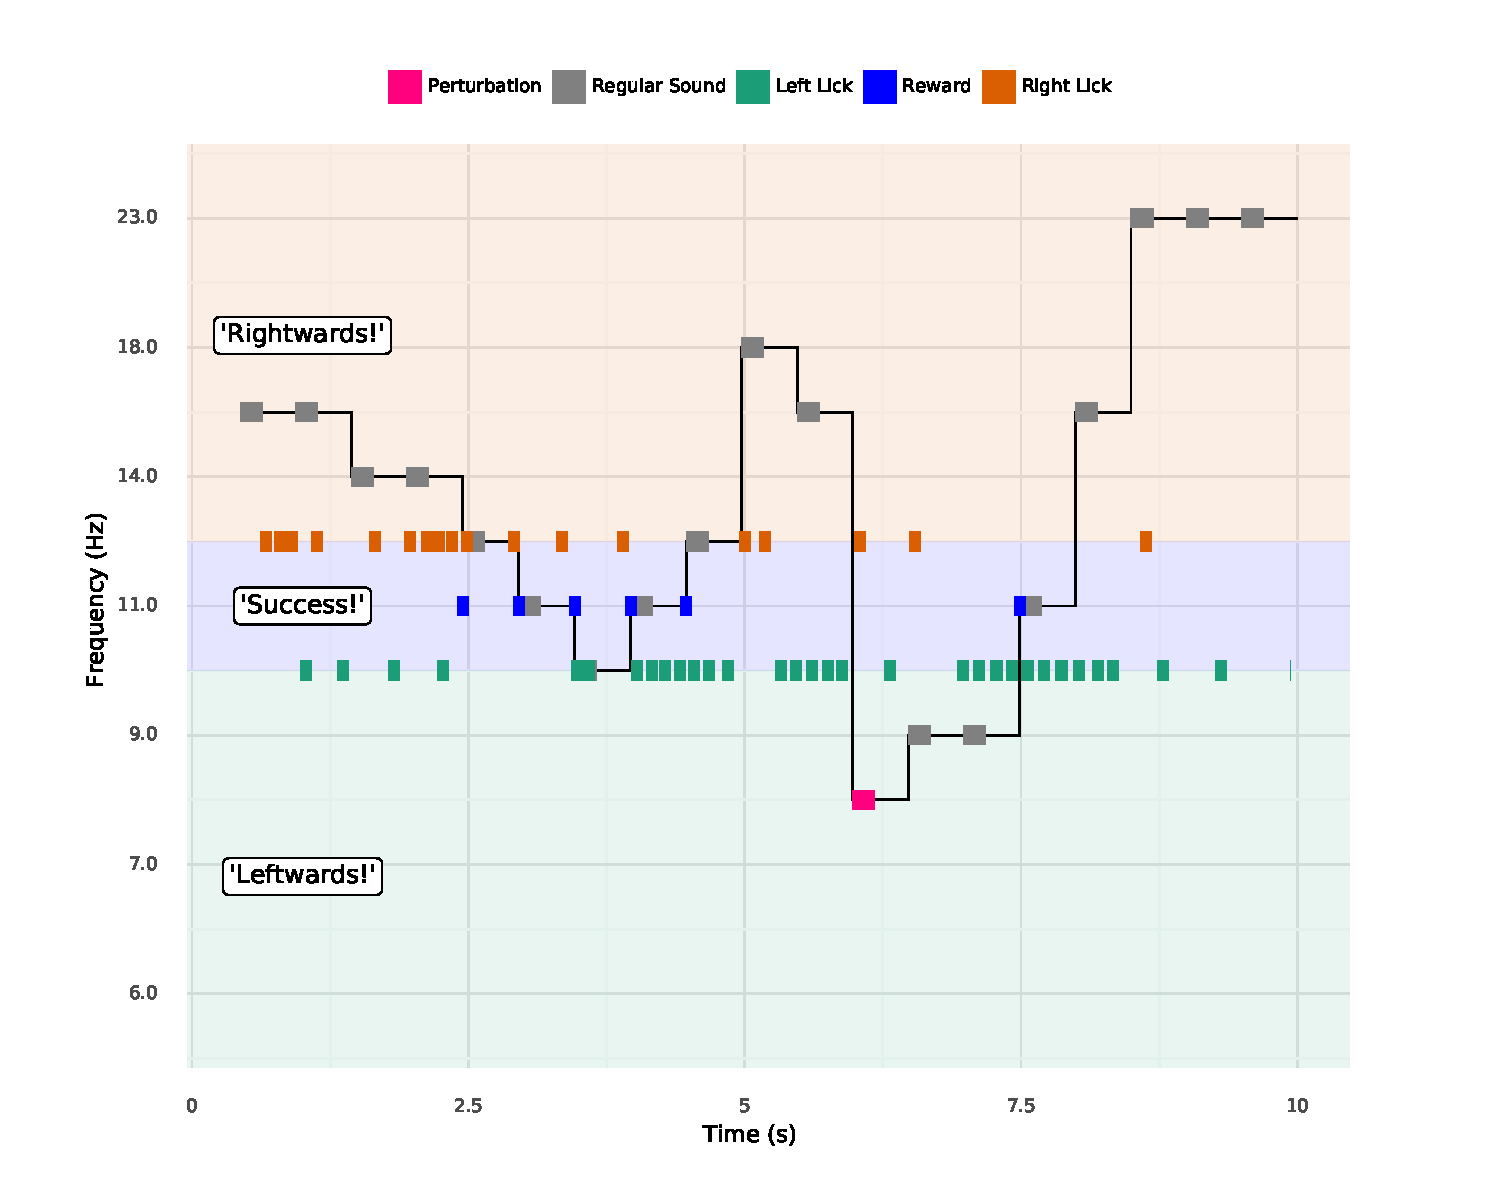
\includegraphics[width=0.9\linewidth]{thesis-tt-19_files/figure-latex/a-example-py-1} 

}

\caption{An example sequence of M10 undergoing the behavioural
task. The gray tiles visualize the unperturbed presented stimuli. The
time of stimulus presentation is shown on the x axis and their frequency
in kHz is shown on the y axis. Pink tiles illustrate a perturbed sound.
Furthermore, green tiles indicate left licks, orange tiles indicate
right licks. Blue tiles indicate rewards.}\label{fig:a-example-py}
\end{figure}








Based on the above reasoning we can assess whether the animal's
behaviour is compatible with a sound-driven policy. In the example
sequence, this is the case so far. However, it is not clear from this
analysis alone that the changing sounds actually determine the lick
strategy. Instead, the mouse might have learned a simple motor pattern
of alternating between left and right lick bouts (henceforth called a
switch policy). An animal simply switching between left and right
licking independently of the sounds could nevertheless be regularly
traversing the target region and therefore receive plenty of rewards.

By introducing targeted violations of the sensorimotor contingency, it
was possible to analyse whether a switch policy alone could account for
the behaviour. In some cases, such a violation led to a `strategy
perturbation', as can be seen in figure \ref{fig:a-example-py}. By
licking left, the animal had reached a `Rightwards!' stimulus. Both a
sound-driven and a motor-driven policy would suggest to lick right.
However, due to a strategy perturbation, the stimulus suddenly jumps to
a `Leftwards!' sound, even though the normal sensorimotor contingency
would have led to a `Rightwards!' sound. The motor-driven policy would
therefore erroneously suggest to switch and lick right, whereas a
sound-driven policy would correctly suggest to not switch and continue
to lick left. Strategy perturbations can therefore be used to
distinguish between a switch policy and a sound-driven policy.

Of course, a different motor-driven policy could cause the mouse to
correctly react to strategy perturbations, namely by continuously
licking on one side. However, this policy would fail to provide the
mouse with any rewards when no perturbations occur. Only a sound-driven
strategy can account for the correct lick pattern in both cases. By
comparing the effect of violations that lead to a strategy perturbation
to those that do not, it is therefore possible to assess whether the
mice have learned the sensorimotor contingency.

\hypertarget{lickrates-after-a-strategy-change}{%
\subsection{Lickrates after a strategy
change}\label{lickrates-after-a-strategy-change}}

For the purpose of such a comparison, this section will analyze
lickrates before and after sounds that imply a change in strategy, as
well as before and after strategy perturbations, using M10 as an
example. It is important to note that this mouse (like most others) was
generally more likely to lick the left than the right spout.\footnote{The
  consistent left bias might be explained by the position of the headbar
  and the cranial window that was also consistent across all animals.
  The added weight of these implants require compensatory mechanisms by
  the animals that might have induced the bias as a side effect.}

As figure \ref{fig:strategy-change} demonstrates in the case of mouse
M10, a change in strategy is preceded by licking of the opposite spout,
as this drives the sound into the corresponding region. Furthermore, it
is followed by an increased lick rate in the direction that is suggested
by the stimulus. This increase is pronounced for a `Leftwards!' event
and more attenuated -- but nonetheless present -- in the case of a
`Rightwards!' event. It begins about 500 ms before the sound that causes
a strategy change and reaches its peak within 500 ms after that sound.

\begin{figure}

{\centering 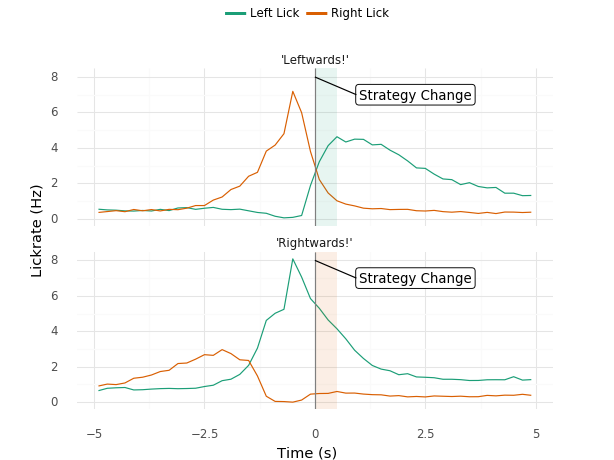
\includegraphics[width=0.9\linewidth]{thesis-tt-19_files/figure-latex/strategy-change-1} 

}

\caption{The lick rate before and after a sound that
changes the appropriate strategy either to `Leftwards!' (upper panel) or
`Rightwards!' (lower panel). Data has been averaged across all sessions
by M10.}\label{fig:strategy-change}
\end{figure}






The animal therefore reacted to a strategy change in the appropriate
manner. This reaction was either sound-driven or due to a learned switch
pattern. In particular, this animal often started an active phase (i. e.
a phase with a high lick rate) with a right lick bout that was followed
by a left lick bout. In order to investigate whether such a motor
pattern can explain away the animal's behaviour, figure
\ref{fig:a-lickrates} visualizes the average lick rates of M10 centered
around violations of the contingency that either perturbed the current
strategy (henceforth called `perturbation' events, see figure
\ref{fig:a-example-py}) or did not perturb the current strategy (`no
perturbation').

\begin{figure}

{\centering 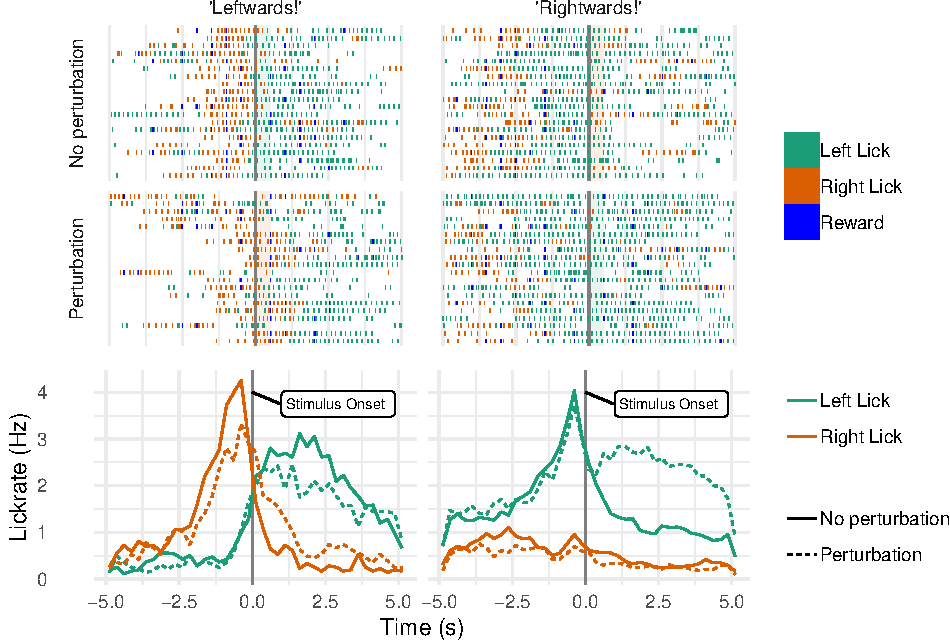
\includegraphics[width=1\linewidth]{thesis-tt-19_files/figure-latex/a-lickrates-1} 

}

\caption{The top panel depicts, in a raster plot, example
events centered around perturbed and unperturbed events. The bottom
panel shows the lickrate histogram centered around these events for M10.
The x axis shows the time centered around stimulus onset and the y axis
shows the lickrate. On the left side, events where the sensorimotor
contingency led to a `Leftwards!' sound are depicted. In the
no-perturbation case, the new sound still suggested a left lick bout. In
the case of a perturbation event, the new sound suggested to lick right.
On the right side, events where the sensorimotor contingency led to a
`Rightwards!' sound are depicted. Similarly, the no-perturbation case
does not change this strategy, whereas the perturbation case does.}\label{fig:a-lickrates}
\end{figure}













These violations only occurred during periods when the animals were
actively engaged in the task, i.e.~when the lick rate was non-zero in
the immediate past, but were otherwise random. Restricting the analysis
to those stimuli that represented a violation of the contingency
therefore made the history between perturbation events and
no-perturbation events comparable. As expected, the lick rates preceding
stimulus onset were similar for both types. The only notable difference
is given by an elevated right lick rate in the event of a `Leftwards!'
strategy without perturbation.

The behavioural pattern following a no-perturbation event was consistent
with the pattern following a strategy change within the sensorimotor
contingency. In contrast, a perturbation of the strategy led to an
immediate change of the left lickrate into the appropriate direction. If
a `Leftwards!' sound changed to a `Rightwards!' sound, the left lick
rate that had already started ramping up instantly decreased again. In
the case of the reverse change, the left lick rate interrupted its quick
decrease and instead increased again. Though less severely, the right
lick rate changed in the appropriate manner, as well. The strategy
perturbation therefore broke the regular switch pattern.

This response was not driven by random fluctuations. This could be
confirmed by using a nonparametric test to compare the lick rates in the
second before and after stimulus onset and comparing them between events
that led to a strategy change and those that did not (see figure
\ref{fig:a-significance}).In three out of four types of events, the
licking behaviour of M10 before stimulus onset showed no significant
differences between perturbation and no-perturbation events
(\(U=(8380, 95448, 105208)\), \(p = (0.74, 0.20, 0.11)\)). However, for
a `Leftwards!' strategy, right lick rates were significantly elevated in
the event of perturbations compared to no perturbations (\(U=6418\),
\(p=0.0025\)).

\begin{figure}

{\centering 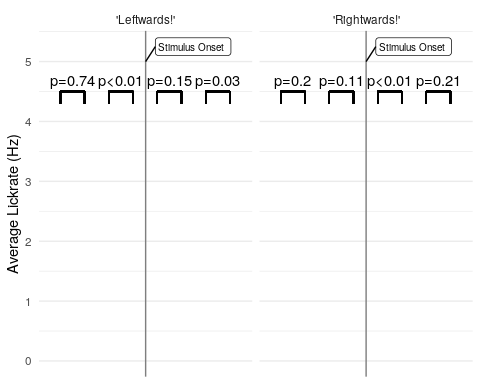
\includegraphics[width=0.9\linewidth]{thesis-tt-19_files/figure-latex/a-significance-1} 

}

\caption{The differences in lickrates as a result of
perturbation and no-perturbation events and the significance of their
difference according to a Mann-Whitney U test.}\label{fig:a-significance}
\end{figure}





In contrast, after a strategy perturbation, the lickrates into the
direction of the perturbation significantly increased when compared to
their level during a non-perturbed event in which licks into this
direction were not necessary (\(U=(9230,111039)\),
\(p=(0.032, 0.0025)\)). The lickrates into the previous direction
decreased in the event of a perturbation, but those changes were not
significant (\(U=(8814, 102516)\), \(p=(0.15, 0.21)\)).

These results demonstrate that lick strategies cannot be fully explained
by a motor-driven policy, and are at least partly explained by a
sound-driven policy. Therefore, we can conclude that M10 has acquired
the sensorimotor contingency.

This analysis can be further summarized by determining and comparing the
change in lick rate difference elicited by the different types of
events. This change is defined as the difference between the right and
left lick rate in the second after stimulus onset compared to the lick
rate difference in the second before stimulus onset. A positive (resp.
negative) change in lick rate difference therefore suggests that the
proportion of right (resp. left) licks was higher following stimulus
onset. Compared to regular sounds, strategy perturbations shifted this
change in lick rate difference significantly into the correct direction
in mouse M10 (\(\chi^2=13.5\), \(p=0.00012\)).

\hypertarget{group-analysis-of-behavioural-learning}{%
\subsection{Group analysis of behavioural
learning}\label{group-analysis-of-behavioural-learning}}

The Prentice-Wittkowski test comparing changes in lickrate difference
allowed for a compact assessment whether a mouse had learned the task
using a sound-driven policy and indicated that five out of nine mice had
learned to employ such a policy and therefore had acquired the
contingency (see \ref{tab:significance}). The average reactions to a
strategy perturbation can be found in the appendix.

\begin{table}[t]

\caption{\label{tab:significance}Table summarizing the results of the
Prentice-Wittkowski test for each mouse, specifying the result in terms
of the test statistic \(\chi^2\) and the p-value.}
\centering
\begin{tabular}{lrr}
\toprule
Mouse & Test Statistic & p-value\\
\midrule
M01 & 1.1000 & 0.86000\\
M03 & 0.0033 & 0.52000\\
M04 & 0.5700 & 0.23000\\
M06 & 9.5000 & 0.00100\\
M07 & 3.0000 & 0.04200\\
\addlinespace
M08 & 6.5000 & 0.00530\\
M09 & 0.0021 & 0.48000\\
M10 & 13.0000 & 0.00012\\
M11 & 9.6000 & 0.00096\\
\bottomrule
\end{tabular}
\end{table}





\hypertarget{course-of-learning}{%
\subsection{Course of learning}\label{course-of-learning}}

In mouse M10, which performed this task for twenty days, this
sound-driven policy emerges over the course of training. By splitting
its sessions up into the first (days one to seven) and last (days
fourteen to twenty) third, it is possible to study the evolution of the
sound-driven policy (figure \ref{fig:course}).

\begin{figure}

{\centering 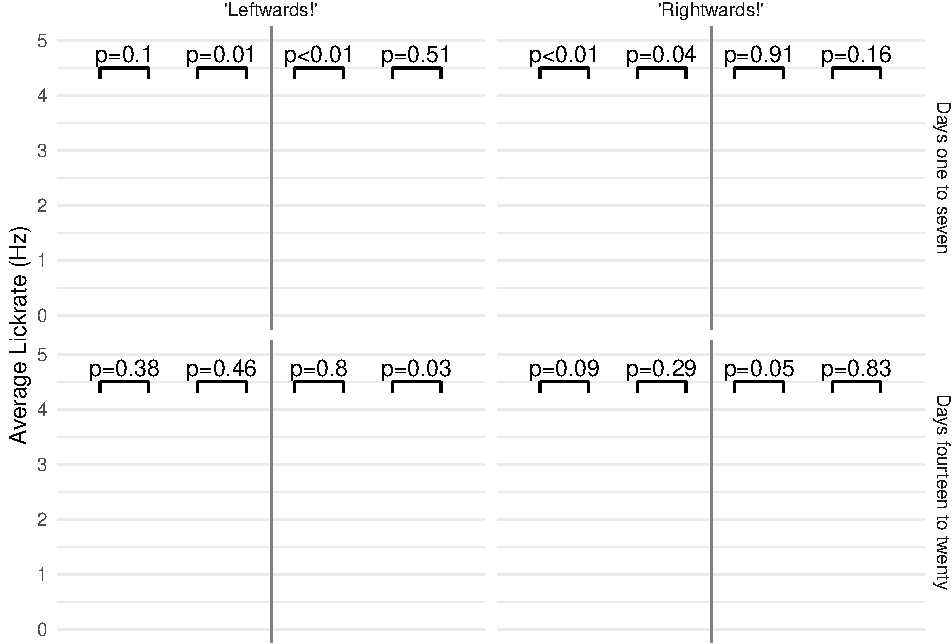
\includegraphics[width=0.9\linewidth]{thesis-tt-19_files/figure-latex/course-1} 

}

\caption{The top panels illustrate the differences in lickrates of
M10 as a result of perturbation and no-perturbation events and the
significance of their difference across the first seven days. The bottom
panels illustrate that difference at the end of the behavioural
training. The lineranges reflect 95\% confidence intervals.}\label{fig:course}
\end{figure}







The most important response to strategy perturbations, the increase of
the lickrate in the appropriate direction, is not significant in the
first seven days (\(U=(1141,8050)\), \(p=(0.51, 0.91)\)), but is in the
last seven (\(U=(764,11090)\), \(p=(0.03,0.05)\)). In contrast, the left
lickrate is already significantly attenuated in the appropriate event
within the first seven days (\(U=1450\),\(p=0.0080\)).\footnote{It is
  important to note here that the first seven days contain few
  perturbations. This might be an explanation for the discrepancy
  between the overlapping confidence intervals and the significant
  Mann-Whitney U test, which evaluates a rank sum rather than a
  difference of means.} In the last seven days, neither the right nor
the left lickrate are significantly attenuated for perturbations that
suggest a strategy in the opposite direction (\(U=(544,9512)\),
\(p=(0.80,0.83)\)). Overall, however, the behaviour of M10 can be better
explained by a sound-driven policy for the last seven days compared to
the first seven days, indicating an improvement in performance over
time. This is supported by a Prentice-Wittkowski test applied to the
first and the last seven days. While this test is significant in both
cases, the test statistic is higher and the p value smaller at the end
of the behavioural training (Days one to seven: \(\chi^2=3.17\),
\(p=0.038\); Days fourteen to twenty: \(\chi=20.8\), \(p=2.6e-6\)).

By assessing the change in lick rate difference that the four different
kinds of strategy perturbations evoke on a daily basis, the emergence of
the sensorimotor behaviour over time can be studied in a more detailed
manner (figure \ref{fig:lrd}). If the animal behaves in a sensible
manner, this change in lick rate difference should be positive (resp.
negative) if the sound suggests a `Rightwards!' (resp. `Leftwards!')
strategy. Within the first couple of days, the change in lick rate
difference in response to no-perturbation `Leftwards!' events quickly
reached a strong negative value. Compared to that the change in lick
rate difference in response to no-perturbation `Rightwards!' events rose
more slowly. In a perturbed `Leftwards!' event suggesting a right lick
bout, the initial response appeared similar to a non-perturbed
`Leftwards!' event. Over time, however, compared to the regular
reaction, this change in lick rate difference shifted towards a higher
proportion of right licks. A similar, but more subtle pattern emerges
from the perturbed `Rightwards!' events, as well.

\begin{figure}

{\centering 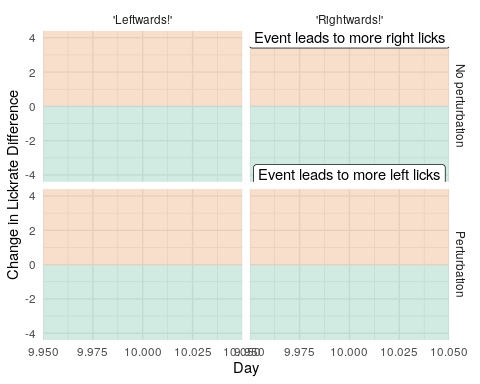
\includegraphics[width=0.9\linewidth]{thesis-tt-19_files/figure-latex/lrd-1} 

}

\caption{The evolution of the change in lick rate difference over
training time.}\label{fig:lrd}
\end{figure}




\hypertarget{representation}{%
\section{Representation}\label{representation}}

This section discusses the evidence that auditory cortex represents the
sensorimotor contingency. For the purpose of this analysis, this is
assumed to be the case if violating the sensorimotor contingency changes
the representation of the presented stimulus. In the previous section,
the contingency was violated with jumps large enough to induce a
strategy change. Auditory cortex represents such sensory oddballs
regardless of their relation to the contingency
\citep{rubin2016representation}. This analysis therefore required more
subtle sensorimotor violations. To distinguish sensory oddball responses
from sensorimotor perturbation responses, events were selected that were
matched in terms of sensory statistics, but differed from regular sounds
in as far as they violated the sensorimotor contingency. Sensory
statistics were assumed similar if the previously and currently
presented stimuli were equal across both conditions.

If auditory cortex is sensitive to such subtle perturbations, this would
therefore suggest that the area takes motor evidence into account in a
contingency-specific manner. By recording single-neuron responses in
auditory cortex while the mouse was engaged in the task and occasionally
presented with perturbations, it was determined whether auditory cortex
was sensitive to violations of the sensorimotor contingency.

\hypertarget{frequency-tuned-neurons-in-auditory-cortex}{%
\subsection{Frequency tuned neurons in auditory
cortex}\label{frequency-tuned-neurons-in-auditory-cortex}}

As a first step, neurons were identified that were sensitive to the
presented tones. In primary (A1) and secondary (A2) auditory cortex as
well as the anterior auditory field (AAF), neurons are globally
organized in a topographical manner according to their best frequency,
i. e. the sound frequency they respond to most strongly
\citep{stiebler1997topographic, bizley2005functional, issa2014topographic}.
Using widefield imaging, the location of the cranial window over
auditory cortex was confirmed and the locations of A1, A2, and AAF were
determined (figure \ref{fig:frequency-tuning}a). While the mice
performed the behavioural task, we recorded the activity from individual
neurons in layer 2/3 (170-250µm depth) of these regions using 2-photon
calcium imaging and determined the deconvolved spike rate using the
`suite2p' algorithm \citep{pachitariu2017suite2p}. This section analyses
an example session in L2/3 (-205µm) of putative A1 in mouse M10.

After determining the average spike rate in response to a presented
stimulus, neuronal frequency tuning was determined using the
Kruskal-Wallis statistic, a nonparametric version of the analysis of
variance \citep{kruskal1952}. The neurons with the strongest frequency
tuning (\(p<0.0001\)) were selected for further analysis. Most of the
selected neurons showed typical frequency tuning curves (figure
\ref{fig:frequency-tuning}b,c) and a typical average response to sound
presentation (figure \ref{fig:frequency-tuning}d), with a mixture of
onset and offset responses \citep{qin2007offset, liu2019offset}.

\begin{figure}

{\centering 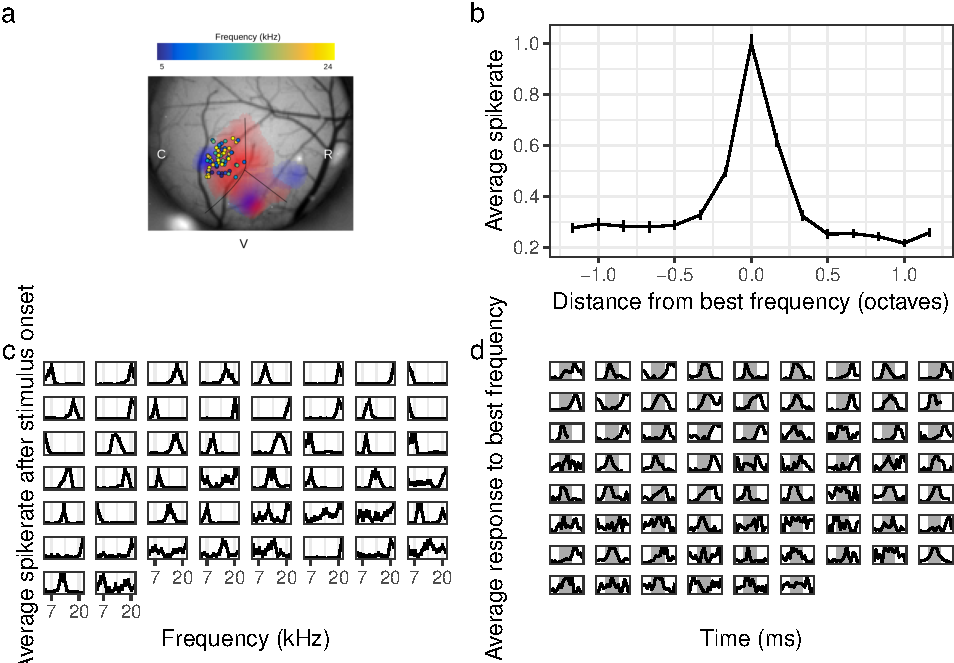
\includegraphics[width=0.95\linewidth]{thesis-tt-19_files/figure-latex/frequency-tuning-1} 

}

\caption{Frequency tuning in auditory cortex. \textbf{a}
The recorded area in mouse M10. Shaded areas are pixels with significant
responses (z-score\(>1\)) to 4 kHz (blue) and 25 kHz (red) SAM tones.
Putative boundaries between A1 (left), AAF (bottom), and A2 (right) are
indicated. Frequency-tuned neurons are shown shaded according to their
best frequency (kHz). \textbf{b} Average tuning curve centered around
the best frequency of all neurons. Lines indicate 95\% confidence
intervals. \textbf{c} Tuning curves with 95\% confidence intervals of
the most strongly tuned neurons as measured by a Kruskal-Wallis test.
Frequency varies along the x axis and spike rate varies along the y
axis. The scale of the y axis is not consistent across neurons and has
been omitted for clarity. \textbf{d} Average spike rates in response to
a best-frequency stimulus presented for 200 ms (represented by the
shaded block). Time varies along the x axis and spike rate varies along
the y axis. Again, the scale of the y axis is not consistent across
neurons and has been omitted for clarity.}\label{fig:frequency-tuning}
\end{figure}


















\hypertarget{sensorimotor-perturbations}{%
\subsection{Sensorimotor
Perturbations}\label{sensorimotor-perturbations}}

This section evaluates whether auditory cortex represents the
sensorimotor contingency. This would be the case if the stimulus
representation was different for sensorimotor perturbations compared to
sounds that followed the contingency. In order to control for any neural
effects driven by sound history statistics themselves, the responses to
sensorimotor perturbations were compared to non-perturbed sounds with
matched frequency and stimulus history (going back one stimulus).

A Prentice-Wittkowski test over the full population of frequency-tuned
neurons revealed that the spike rates elicited by perturbed stimuli were
significantly different from those following non-perturbed stimuli
(\(\chi^2=5.3\),\(p=0.02\)). This suggests that the population of
neurons recorded in this session indeed represents the sensorimotor
contingency. Overall, the neurons appear more broadly tuned in the event
of perturbed stimuli, though due to the limited sample size, this is
difficult to assess using an averaged tuning curve (figure
\ref{fig:perturbation}d).

\begin{figure}

{\centering 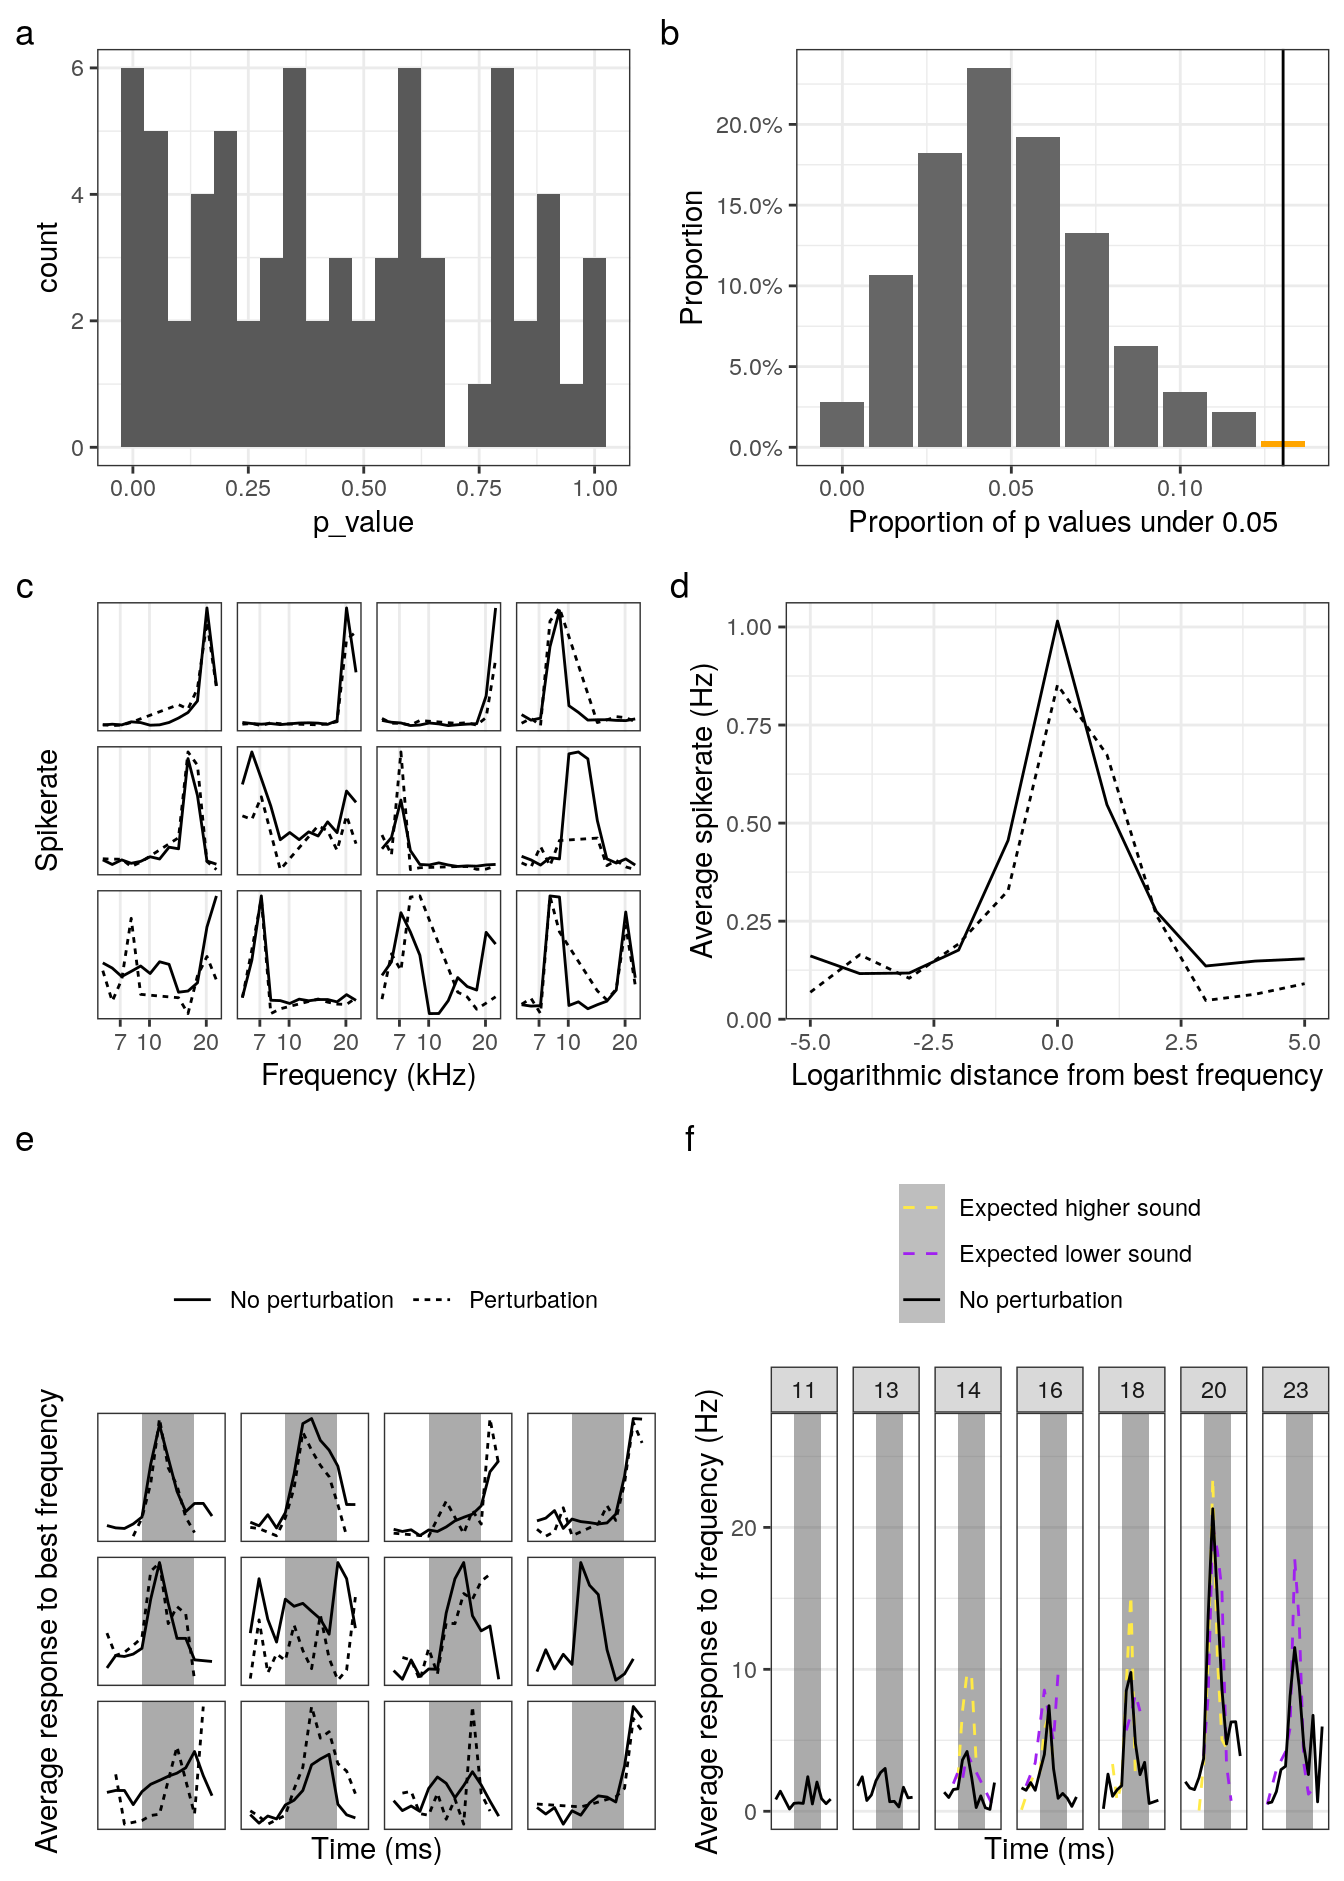
\includegraphics[width=0.9\linewidth]{thesis-tt-19_files/figure-latex/perturbation-1} 

}

\caption{Representation of sensorimotor perturbations.
\textbf{a} Distribution of the p values of the Prentice-Wittkowski test
for each neuron. \textbf{b} Simulated distribution of proportions of p
values under 0.05 if all underlying hypotheses were wrong. The
proportion of p values under 0.05 in the given hypothesis test (marked
in orange) is significantly higher than the null distribution.
\textbf{c} Frequency tuning curves to perturbations and
non-perturbations of neurons that are possibly sensitive to sensorimotor
perturbations. \textbf{d} Average tuning curve around the best frequency
for perturbations and no perturbations. \textbf{e} Average evoked
response of the neurons from panel c, with and without perturbations.
\textbf{f} Tuning curve of an example neuron.}\label{fig:perturbation}
\end{figure}














Next, the representation of sensorimotor perturbations was considered at
the level of individual neurons. Applying the Prentice-Wittkowski test
to single neurons yielded nine out of 69 frequency-tuned neurons with a
p value of under 0.05.\footnote{Note that on a neuronal level, the test
  has much less statistical power due to the strongly reduced sample
  size.} This was a higher number than what would have been expected due
to random fluctuations: a permutation test with shuffled perturbations
led to nine or more perturbation-sensitive neurons in less than 0.02\%
of the cases (i. e. p=0.0002) (figure \ref{fig:perturbation}b). This is
further evidence that auditory cortex indeed represents sensorimotor
perturbations.

Inspection of the neurons that were the most sensitive to perturbations
reveals that in some cases, the perturbation modulated the amplitude of
the neuronal response without affecting the frequency tuning, whereas in
other cases, the response to sensorimotor perturbations was shifted in
frequency. Figure \ref{fig:perturbation}e visualizes the average
response to a best-frequency stimulus that represents or does not
represent a perturbation. In many cases, the perturbation modulates the
response, either by making it stronger or weaker. However, other effects
can be found as well. In particular, one example neuron showed a broader
frequency tuning to sensorimotor perturbations (figure
\ref{fig:perturbation}f). Indeed, it was particularly sensitive to
events whose expected sound was near the best-frequency stimulus,
suggesting that it responded to a mixture of the presented and expected
sound.

In this manner, inspection of single neurons can shed light on possible
mechanisms by which sensorimotor perturbations are represented. The
analysis presented here does not allow us to validate or reject such
hypothesized mechanisms. At this stage, however, it is possible to
confirm that neurons in auditory cortex represented, in some way,
sensorimotor perturbations differently from sounds within the
contingency.

\hypertarget{discussion}{%
\chapter{Discussion}\label{discussion}}

In this dissertation, mice were trained on a novel sensorimotor task
relating their licking behaviour to continuous auditory feedback. This
dissertation focussed on analysing the acquired behavioural data, and
the cortical representation in mouse M10 during one day of imaging.
These data demonstrate that five out of nine analysed mice (including
M10) learned the sensorimotor contingency and they suggest that the
contingency was represented by neurons of the primary auditory cortex.

\hypertarget{behavioural-evidence-for-task-acquisition}{%
\section{Behavioural evidence for task
acquisition}\label{behavioural-evidence-for-task-acquisition}}

In the novel behavioural task, the mouse could manipulate the frequency
of the presented tone sequence by licking one of two spouts. They were
rewarded with a small drop of water if they moved the stimulus into a
particular frequency region. At any given time, the spout the animal
should lick was therefore determined by the presented stimulus.

Mouse M10 reacted to the presented stimuli by increasing its lickrate in
the corresponding direction. Due to the continuous integration between
motor behaviour and subsequent stimulus presentation, however, a
motor-driven policy (i.e.~switching every few seconds between left and
right lick bouts) would allow the animal to receive plenty of rewards
under the regular contingency. The resulting behavioural pattern would
be indistinguishable from a behavioural pattern emerging from a
sound-driven policy. Whereas the reaction of M10 to the normal paradigm
was therefore a necessary condition for a sound-driven policy, it was
not sufficient evidence.

Importantly, this analysis suggests that the policy was at least in part
driven by the presented stimuli. It might, however, also have included a
learned motor pattern.

The analysis does not allow for a distinction between two alternative
sound-driven policies. On the one hand, the data could be explained by
an associative mechanism whereby the animal learned to lick into a
certain direction as a response to the presented sounds, but did not
take into account how this licking behaviour changed this stimulus
presentation. On the other hand, an integrated mechanism would propose
that the animal learned to navigate in a one-dimensional tonespace using
left and right licks, and used this rule to reach a rewarded frequency
region. The manner in which the task was constructed aimed to make the
implementation of an integrated (rather than associative) sound-driven
policy more likely. In particular, this was the reason why the
contingency was not presented in a trial-based manner, as this would
have led the animal to focus on purely learning a behavioural response
to a presented stimulus. In contrast, the continuous task approach
allowed the animal to move freely in this integrated virtual
environment, and to be in near-complete control of its sensory feedback.
How the two sound-driven policies could be distinguished using both
acquired data and further variations of the experiment will be discussed
below.

\hypertarget{auditory-cortex-represents-the-artificial-sensorimotor-contingency}{%
\section{Auditory cortex represents the artificial sensorimotor
contingency}\label{auditory-cortex-represents-the-artificial-sensorimotor-contingency}}

Sensory cortex has been found to change its tuning properties in
accordance with task demands, allowing for enhanced perceptual
discrimination as well as qualitative changes in the representation of
task-related stimuli
\citep{jeanne2013associative, peron2015whiskers, chu2016balancing}. In
order to investigate the role of sensory areas of the cortex in task
acquisition, we recorded from neurons in auditory cortex of mice while
they were engaged in the task. In this dissertation, one example session
in M10 was analysed.

Neurons in auditory cortex encode a reduced representation of stimulus
history \citep{rubin2016representation}. In order to control for this
effect regular stimuli were compared to contingency violations that were
otherwise fully matched in recent sensory statistics. On a population
level, the representation of these sounds was significantly different.
Single-neuron analysis revealed that this effect was driven by a strong
difference in the responses of a small proportion of recorded neurons.

Furthermore, the analysis suggested possible mechanisms by which this
representation might operate. In particular, the tuning curves derived
from perturbed sounds appeared broader than the regular tuning curves.
This is consistent with a model where certain neurons represent a
mixture of expected and presented sounds, shifting their responses away
from the presented sounds in the event of an unexpected event. In
particular, one example neuron exhibited exactly this kind of pattern:
Compared to its best-frequency it fired more strongly in response to a
perturbation leading to a lower-frequency stimulus if the expected sound
was higher and vice versa.

A clearer picture of these representational patterns will be determined
using further imaging data. With a larger sample size, it would for
example be possible to estimate a mathematical model of how neurons in
auditory cortex represent quantities related to the sensorimotor
contingency such as expected frequency and prediction error.

\hypertarget{implications-of-the-behavioural-and-neural-analysis}{%
\section{Implications of the behavioural and neural
analysis}\label{implications-of-the-behavioural-and-neural-analysis}}

Combined, behavioural and neuronal evidence suggests that it is possible
to train head fixed mice on a behavioural task that is based on an
artificial sensorimotor contingency, leading to a cortical
representation of this contingency. From a computational perspective,
such a task has important implications for general theories of
sensorimotor learning and intelligence. Methodologically, the fact that
this computationally rich task can be applied to head fixed mice means
that its neural correlates can easily be studied using 2-photon imaging
and other techniques that currently cannot be applied to freely moving
animals.

As a next step, the behavioural data in the other animals will be
analysed to determine whether they have learned the task. Furthermore,
the representation of the contingency and the manner in which sensory
and motor evidence are integrated will be investigated within the
available neuronal dataset. Below, I will elaborate on how the collected
data can be used for such investigations and propose extensions of the
task paradigm that would shed light on questions that are currently not
within reach.

In computational theories of intelligence, solving more complex tasks
often involves a tradeoff between two important principles of learning.

On the one hand, by extracting statistical patterns from our
environment, we learn about the information we should take into account
to solve these tasks. This applies to sensory statistics as well as
sensorimotor contingencies. The general smoothness of objects can be
used to parse information at subneuronal \citep{srinivasan1982pc} and
neuronal level \citep{rao1999pc}. This representation is apparent in all
sensory modalities \citep{fox2005comparison, smith2006efficient} and is
sensitive to artificial manipulations of sensory statistics
\citep{wood2016chick, wood2018chick}. In a sensorimotor context,
corollary discharges allow for sensory consequences of motor behaviour
to be cancelled out. This is mediated, in part, by auditory cortex
\citep{schneider2014discharges} and is sensitive to artificial
contingencies, as well \citep{schneider2018cortical}.

On the other hand, the ultimate goal of neuronal processes is to
generate appropriate behaviour. Following this perspective, the brain
should gradually discard task-irrelevant information to optimize
behavioural output. This idea is reflected in receptive fields in
sensory cortex
\citep{hubel1965receptive, hubel1968receptive, aertsen1980receptive, aertsen1981receptive},
which can reshape their properties according to task-relevance
\citep{fritz2003rapid}, and extends to more complex tasks such as object
recognition in the ventral stream \citep{dicarlo2012visual} and semantic
development in humans \citep{saxe2019semantic}.

The presented task lies at the interface of these two theories. On the
one hand, the goal of the task is ultimately to receive a reward in the
form of water. On the other hand, this goal can more easily be reached
by recognizing the sensorimotor contingency. Since neural data suggests
that auditory cortex represents this contingency and this area is also
involved in shaping behavioural learning, it appears likely that the
animal's behaviour is indeed not only driven by auditory associations,
but in particular implements a contingency-driven behavioural policy.

Whether behavioural relevance has an impact on the extraction of
sensorimotor contingencies in sensory cortex could be probed by making
the rewards only contingent on the number of licks, leading the mice to
explore the tonespace in any direction, without direct consequences on
the likelihood of reward. This would connect the experiment more closely
with the passive presentation of a novel sensorimotor contingency by
\citet{schneider2018cortical}.

Neurons that are sensitive to pure sensorimotor perturbations are likely
implicated in the integration of sensory and motor evidence. Both
multisensory and sensorimotor integration processes in the brain are
compatible with a Bayesian model and take the uncertainty associated
with the different stimuli into account
\citep{wolpert1995internal, kording2004force, kording2004bayesian, oreilly2012bayesian}.
In order to test whether the contingency representation in auditory
cortex was implicated in a similar mechanism of evidence integration,
the sound levels were modulated on some sessions so as to present
stimuli with different degrees of uncertainty. These level modulations
can be used to probe the purpose of the perturbation-sensitive neurons.
As an example, if the neuron in figure \ref{fig:perturbation}b indeed
represents a mixture of the presented and expected sound, the neuron's
tuning curve would be shifted closer to the expected rather than the
presented sound for less certain, i. e. more silent auditory input.
Extensions of this idea might manipulate precision of the auditory
stimuli by increasing their bandwidth or presenting several stimuli at
once.

Similarly to the neuronal representation, the existence of an internal
model can be tested behaviourally by manipulating the precision of the
provided information \citep{wolpert1995internal}. This would allow for a
behavioural examination of whether the mice take the sensorimotor
contingency into account when solving the task. The neural evidence of a
representation of the contingency in auditory cortex, an area that plays
a role in behavioural learning, would suggest that this contingency can
affect the mouse's behaviour as well.

When freely moving rats were presented with a similar tonespace,
recordings of the entorhinal-hippocampal circuit provided evidence for
the emergence of grid cells representing this tonespace
\citep{aronov2017grid}. Grid cells had initially been identified as a
neural correlate of invariant spatial behaviour \citep{hafting2005grid}.
More recently, they have also been implicated in non-spatial cognitive
tasks \citep{constantinescu2016grid}, which provides support for the
hypothesis that conceptual knowledge is organized in `cognitive maps'
\citep{tolman1948map}. The emergence of grid cells in this behavioural
task could be tested by determining the anatomical connections of the
neurons representing sensorimotor perturbations and subsequently imaging
entorhinal cortex in behaving mice \citep{low2014entorhinal}.
Furthermore, grid cells generate a particularly precise error-correcting
code compared to classical population codes in sensory cortex
\citep{sreenivasan2011grid}. A better understanding of the
representation of sensorimotor perturbations, which require such an
error correction, might therefore shed light on the emergence of
conceptual grid cells as well.

For the purpose of dissecting the circuit mediating this potential
contingency representation, it would also be important to image
inhibitory neurons in auditory cortex, as the proposed mechanism would
involve cancelling out predictions from another cortical area
\citep{larkum1999inhibition}.

In conclusion, this dissertation presented a new behavioural task for
head-fixed mice involving the learning of a novel, continuous auditory
sensorimotor contingency. Mice were able to learn this task, and neural
data suggest that auditory cortex can represent the corresponding
contingency. As a next step, the variations in the collected data will
allow for a more detailed examination of the implemented behavioural
policy, the representation of the contingency, and the manner by which
the sensory and motor evidence is integrated to guide behaviour.
Furthermore, variations of the task would allow for an examination of
the influence of behavioural relevance on the possible emergence of an
abstract tonespace, connecting a simple task in head fixed mice to some
of the most debated computational theories of learning.

\hypertarget{appendix-appendix}{%
\appendix}


\pagebreak
\phantom{M}
\vfill
\begin{Huge}
\textbf{Appendix}
\end{Huge}
\vfill
\thispagestyle{empty}

\hypertarget{licking-behavior-of-all-mice}{%
\chapter{Licking behavior of all
mice}\label{licking-behavior-of-all-mice}}

\begin{figure}

{\centering 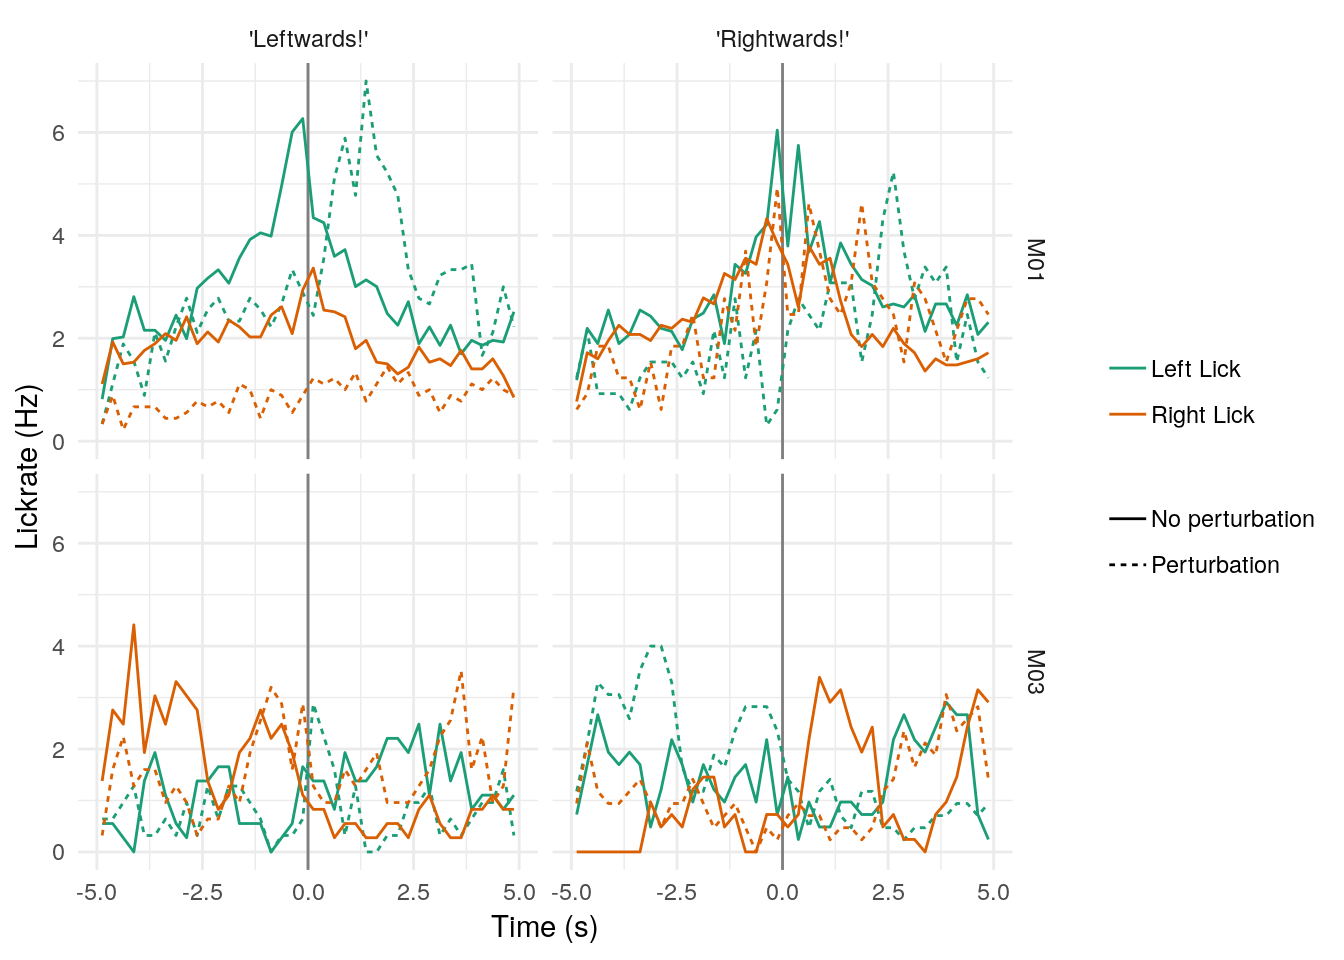
\includegraphics[width=0.9\linewidth]{thesis-tt-19_files/figure-latex/unnamed-chunk-4-1} 

}

\caption{Reaction of M01 and M03 to strategy perturbations}\label{fig:unnamed-chunk-4}
\end{figure}







\begin{figure}

{\centering 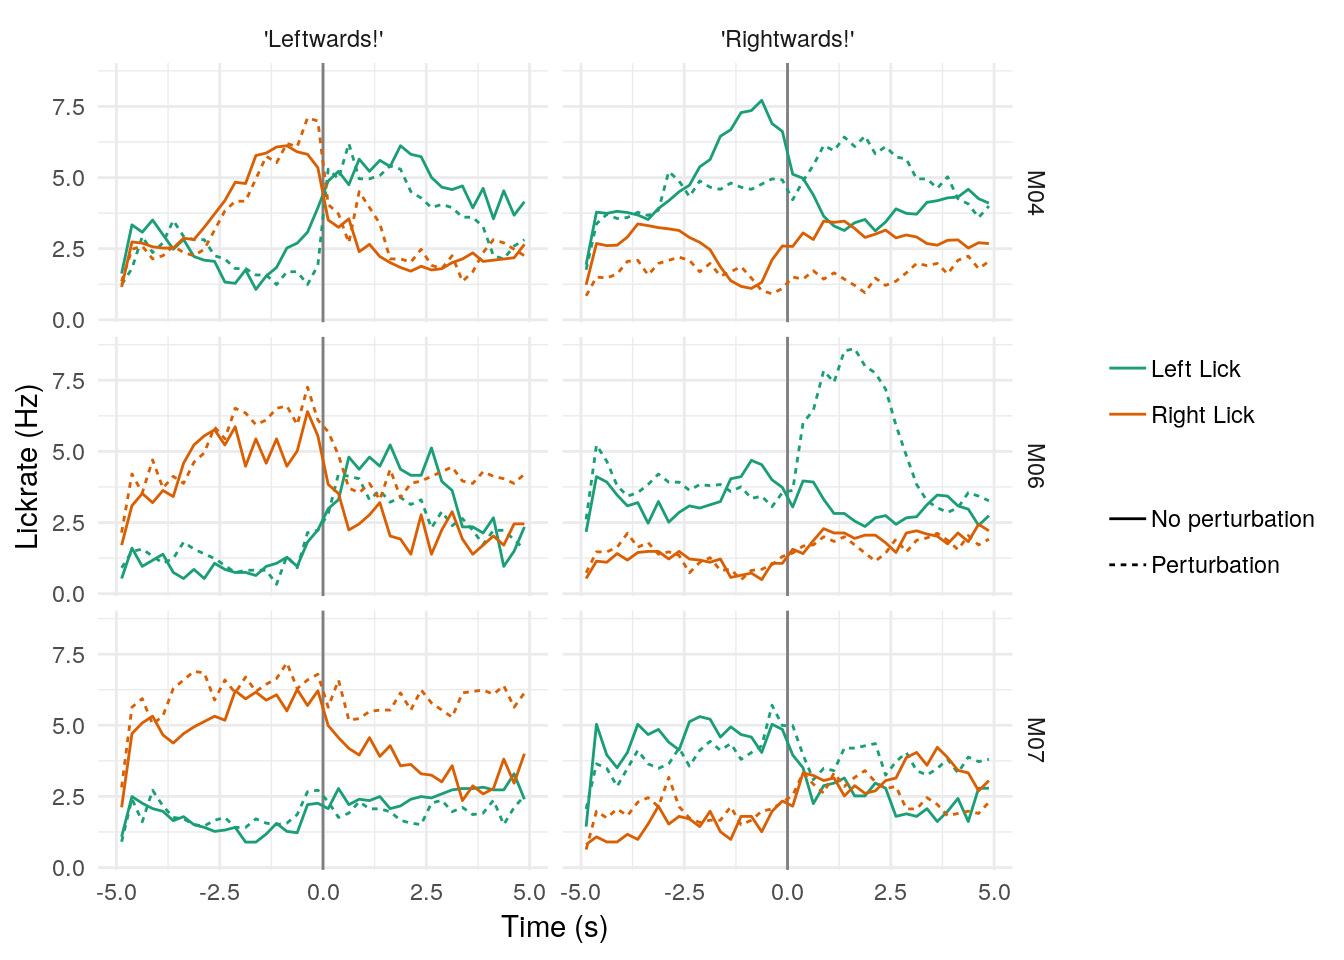
\includegraphics[width=0.9\linewidth]{thesis-tt-19_files/figure-latex/unnamed-chunk-6-1} 

}

\caption{Reaction of M04, M06, and M07 to strategy perturbations}\label{fig:unnamed-chunk-6}
\end{figure}





\begin{figure}

{\centering 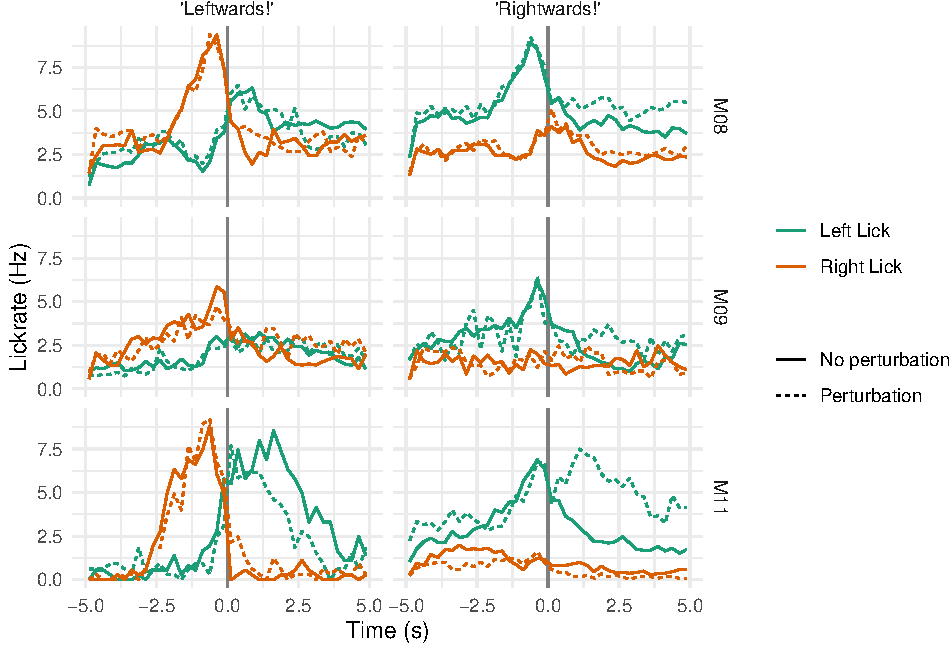
\includegraphics[width=0.9\linewidth]{thesis-tt-19_files/figure-latex/unnamed-chunk-8-1} 

}

\caption{Reaction of M08, M09, and M11 to strategy perturbations}\label{fig:unnamed-chunk-8}
\end{figure}





\bibliography{book.bib,packages.bib}


\end{document}
